\documentclass[12pt,a4paper]{ctexart}

\usepackage{subfigure}
\usepackage[graphicx]{realboxes}
\usepackage{listings}
\usepackage{xcolor}
\usepackage{amsmath}

% (1) choose a font that is available as T1
\usepackage{lmodern}
% (2) specify encoding
\usepackage[T1]{fontenc}
% (3) load symbol definitions
\usepackage{textcomp}

\usepackage{hyperref}

\usepackage{graphicx}

\usepackage{float}

\hypersetup{hidelinks,
	colorlinks=true,
	allcolors=black,
	pdfstartview=Fit,
	breaklinks=true}


\definecolor{mygrey}{rgb}{0.945,0.945,0.945}
\definecolor{myred}{rgb}{1, 0.49, 0.63}

\lstset{
breaklines=true,
 basicstyle=\fontspec{Consolas},
 columns=fixed,       
 numbers=left,                                        % 在左侧显示行号
 numberstyle=\tiny\color{gray},                       % 设定行号格式
 frame=none,                                          % 不显示背景边框
 backgroundcolor=\color[RGB]{245,245,244},            % 设定背景颜色
 keywordstyle=\color[RGB]{40,40,255},                 % 设定关键字颜色
 numberstyle=\footnotesize\color{darkgray},           
 commentstyle=\it\color[RGB]{0,96,96},                % 设置代码注释的格式
 stringstyle=\rmfamily\slshape\color[RGB]{128,0,0},   % 设置字符串格式
 showstringspaces=false,                              % 不显示字符串中的空格
 %language=python,                                        % 设置语言
}
%\def\inline{\lstinline[basicstyle=\fontspec{微软雅黑},keywordstyle={}]}
%opening
\title{The Note of Graph Theory}
\author{Liam}
\date{\today}

\begin{document}

\maketitle

\begin{abstract}
I hate definition!
\end{abstract}

\section{definition}
\begin{center}
    \colorbox{mygrey}{\color{myred}\textbf{simple graph}:}
    \begin{itemize}
        \item a non-empty finite set $V(G)$ of elements \textbf{vertices}
        \item a finnite set $E(G)$ of distinct unordered pairs of deistinct elements \textbf{edges}
        \item at most \textbf{one edge} joining a given pair of vertices
    \end{itemize}
\end{center}
\begin{center}
    \colorbox{mygrey}{\color{myred}\textbf{general graph}:}
    \begin{itemize}
        \item multiple edges
        \item loops
    \end{itemize}
\end{center}
\begin{center}
    \colorbox{mygrey}{\color{myred}graph}
    \begin{itemize}
        \item a non-empty finite set $V(G)$ of elements \textbf{vertices}
        \item a finnite family $E(G)$ of distinct unordered pairs of not necessarily deistinct elements \textbf{edges}
        \item the use of \textcolor{myred}{family} permits the existence of multiple edge
        \item vertex-set  edge-family
    \end{itemize}
\end{center}
$\{v,w\}$ is said to join the vertices v , w and is again abbreviated to $vw$. Example : $vv$ 

\begin{center}
    \colorbox{mygrey}{\color{myred}isomorphism}
    \begin{itemize}
        \item one-one correspondence between the vertices of $G_1$ and those of $G_2$ such that the number of edges joining any two vertices of $G_1$ equals the number of edges joining the corresponding vertices of $G_2$
        \item the \textbf{unlabelled graphs} and \textbf{labelled graphs} is different
    \end{itemize}
\end{center}

\begin{center}
    \colorbox{mygrey}{\color{myred}connected graphs}
    \begin{itemize}
        \item A graph is connected of it cannot be expressed as a union of graghs and disconnected otherwise.
    \end{itemize}
\end{center}

\begin{center}
    \colorbox{mygrey}{\color{myred}Adjacency and degrees(邻接)}
    \begin{itemize}
        \item the $v,w$ is \textbf{adjacency} if there is an edge vw joining them. and $v,w$ are incident with such edge
        \item degree of a vetex is the number of edges incident with itself.
        \item A vetex of degree 0 is an isolated vertex 
        \item A vetex of degree 1 is an end vertex 
    \end{itemize}
\end{center}
The \textbf{degree sequence} of a graph consists of degrees written in \textbf{increasing order}

\begin{center}
    \colorbox{mygrey}{\color{myred}Handshaking lemma}\colorbox{mygrey}{In any graph the sum of all the vertex-degrees}
    \colorbox{mygrey}{is an even number.~~~~~~~~~~~~~~~~~~~~~~~~~~~~~~~~~~~~~~~~~~~~~~~~~~~~~~~~~~~~~~~~~~~~~~~~~~~~~~~~~~~~~~}
\end{center}
\colorbox{mygrey}{\color{myred}Corollary}\colorbox{mygrey}{In any graph the number of vertices of odd degree is even.}
\begin{center}
    \colorbox{mygrey}{\color{myred}Subgraphs}
    \begin{itemize}
        \item A graph is a \textbf{subgraph} of graph G if each of its vertices belongs to $V(G)$ and each of its edges belongs to $E(G)$
        \item we can obtain subgraphs by deleting edges and vertices.
        \item $G-F$
    \end{itemize}
\end{center}

By the way, $G \backslash e$ is the subgraph of G obtained by deleting the edge e 
and $G \backslash v$ is the subgraph of G obtained by deleting the vertex v and all edges incident with it.

\begin{center}
    \colorbox{mygrey}{\color{myred}The complement of a simple graph}
    \begin{itemize}
        \item \textbf{complement} $\overline{G}$ is the simple graph with the same vertex-set as G and with two vertices adjacent in $\overline{G}$ if and only if they are not adjacent in G.
    \end{itemize}
\end{center}

\begin{center}
    \colorbox{mygrey}{\color{myred}Matrix representation of graphs}
~\\
There are two matrix representations of graphs, the \textbf{adjacency matrix} and the \textbf{incidence matrix}.
    \begin{itemize}
        \item \textbf{adjacency matrix} $A(G)$ is the $n \times n$ matrix whose $(i,j)$-entry is 1 if $v_i$ is adjacent to $v_j$ and is 0 otherwise.
        \item \textbf{incidence matrix} $B(G)$ is the $n \times m$ matrix whose $(i,j)$-entry is 1 if $v_i$ is incident with $e_j$ and is 0 otherwise.
    \end{itemize}
\end{center}

\subsection{Examples}

\subsubsection{Null graphs}
A graph whose edge-set is empty is called a \textbf{null graph} 
and is denoted by $N_n$ or simply $N$ if the number of vertices is clear from the context.

\subsubsection{Complete graphs}
A graph with $n$ vertices in which each pair of distinct vertices is joined by an edge is 
called a \textbf{complete graph} and is denoted by $K_n$ or simply $K$ if the number of vertices 
is clear from the context. You can check that $K_n$ has $\frac{n(n-1)}{2}$ edges.

\subsubsection{Cycle graphs, path graphs and wheels}
A \textbf{connected graph} in which each vertex has degree 2 is called a \textbf{cycle graph} 
and is denoted by $C_n$ or simply $C$ if the number of vertices is clear from the context.
You can check that $C_n$ has $n$ vertices and $n$ edges.
\par
A graph obtained from $C_n$ by removing an edge is the \textbf{path graph} $P_n$ or 
simply $P$ if the number of vertices is clear from the context.
\par
The gragh obtained from $C_{n-1}$ by joining each vertex to a new vertex v is the $wheel$,denoted by $W_n$ or simply $W$ if the number of vertices is clear from the context.

\subsubsection{Regular graphs}
A graph is \textbf{regular} if each of its vertices has the same degree. 
If each vertex has degree $r$, the graph is said to be \textbf{r-regular}. 
A \textbf{complete graph} is $r-regular$ for $r=n-1$.
Note that \textbf{cubic graphs} are $3-regular$ graphs, and \textbf{null graphs} are $0-regular$ graphs.

\subsubsection{Platonic graphs}
A \textbf{Platonic graph} is a \textbf{regular} graph with the property that the number of vertices
\begin{figure}[H]
    \centering
    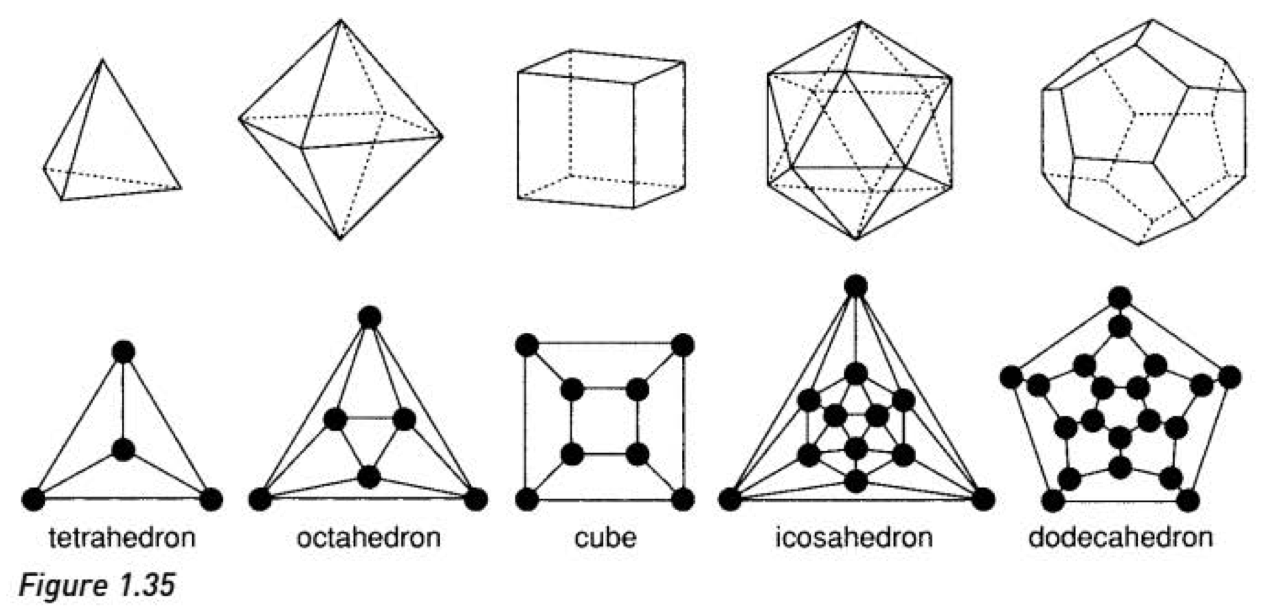
\includegraphics[width=0.5\textwidth]{images/Platonic.png}
    \caption{Platonic graphs}
    \label{fig:platonic}
\end{figure}


\subsubsection{Bipartite graphs}
If the vertex-set of G can be split into two disjoint sets $X$ and $Y$ 
such that each edge of G joins a vertex in $X$ to a vertex in $Y$, 
then G is said to be \textbf{bipartite}.
\par
A \textbf{complete bipartite graph} is a bipartite graph in which every vertex in $X$ is adjacent to every vertex in $Y$ and is denoted by $K_{X,Y}$.

\subsection{Cubes}
The \textbf{cube} $Q_n$ is the graph whose vertices are the $2^n$ binary strings of length $n$





\section{Paths and cycles}
\subsection{Connectivity}
\begin{center}
    \colorbox{mygrey}{\color{myred}Walks}
    \begin{itemize}
        \item A \textbf{walk} in a graph G is a sequence of vertices $v_0,v_1,...,v_n$ such that $v_iv_{i+1}$ is an edge of G for $i=0,1,...,n-1$.
        \item We call $V_0$ the \textbf{initial vertex} and $v_n$ the \textbf{terminal vertex} of the walk.
        \item A \textbf{length} of a walk is the number of edges in it.
        \item A \textbf{closed walk} is a walk in which $v_0=v_n$.
        \item A \textbf{trail} is a walk in which all \textcolor{myred}{edges} are distinct.
        \item A \textbf{path} is a trail in which all \textcolor{myred}{vertices} are distinct.
        \item A \textbf{cycle} is a closed trail in which all vertices are distinct except for $v_0=v_n$.
        \subitem $\circ$ A \textbf{triangle} is a cycle of length 3.
    \end{itemize}

\end{center}

\begin{quote}
    A graph G is bipartite if and only if every cycle of G has even length.
\end{quote}

\end{document}
